\chapter{Implementasi dan Pengujian}

Bab ini akan membahas seluruh proses implementasi yang dilakukan untuk menerapkan rancangan yang sudah didefinisikan sebelumnya. Selain itu, bab ini juga akan membahas pengujian yang dilakukan terhadap hasil implementasi yang mencakup hal-hal yang diuji, metode pengujian, dan hasil pengujian yang diperoleh. 


\section{Implementasi}
Implementasi sistem \textit{Performance Regression Analysis} (PRA) akan dibuat berdasarkan rancangan arsitektur seperti yang terdapat pada gambar \ref{arch-pra}. Beberapa komponen seperti \textit{library} instrumentasi dan juga \textit{User Interface} tidak akan dibuat dari awal, melainkan akan melakukan \textit{fork} dan modifikasi solusi \textit{Open Source} \textit{distributed tracing} dari Zipkin. Komponen yang akan dibuat dari awal sepenuhnya adalah \textit{engine} dari sistem PRA yang akan melakukan komputasi utama sistem pendeteksian dan analisis regresi. Komponen \textit{engine} juga akan berfungsi sebagai API yang akan diakses oleh komponen \textit{User Interface}.



\subsection{\textit{Performance Regression Analysis} \textit{engine}}
Implementasi komponen \textit{engine} ini akan dibagi menjadi beberapa modul, seperti yang terlihat pada tabel \ref{engine-module}.

\begin{small}
	\begin{longtable}{ | p{1cm} | p{3cm} | p{10cm} | }
		\caption{Tabel pembagian modul komponen \textit{engine}}
		\label{engine-module}                                                           
		\\ \hline
		\centering\bfseries{ID} & \centering\bfseries{Nama Modul} & \centering\bfseries{Deskripsi} \tabularnewline \hline
		\endfirsthead
		EM-1 & zipkin (Pengambilan Data) & Modul ini bertanggung jawab untuk mengambil data dari API Zipkin yang memiliki data hasil \textit{trace} dari aplikasi. Selain mengambil data \textit{trace} dari Zipkin, modul ini juga bertanggung jawab untuk mengambil model-model \textit{baseline} yang terdapat pada \textit{storage}. \\ \hline
		EM-2 & transform (Transformasi Data) & Modul ini bertanggung jawab untuk melakukan transformasi dari data \textit{trace} mentah yang diambil dari API Zipkin menjadi bentuk-bentuk model yang akan digunakan untuk komputasi di tahap selanjutnya seperti model \textit{Cumulative Distribution Function} (CDF), model data \textit{Critical Path}, dan sampel data \textit{trace}. \\ \hline
		EM-3 & storage (Penyimpanan Data) & Modul ini bertanggung jawab untuk menyimpan model hasil transformasi \textit{baseline} dari modul EM-2 ke \textit{storage} untuk digunakan kembali pada fase \textit{Real-time Analysis}. \\ \hline
		EM-4 & statistic (Perhitungan Statistik) & Modul ini bertanggung jawab untuk melakukan komputasi perhitungan statistik yang mencakup pendeteksian regresi dengan menghitung koefisien Kolmogorov-Smirnov seperti yang telah dijelaskan pada subbab \ref{approach-cumulative}. \\ \hline
		EM-5 & correlation\textunderscore analysis (Analisis Korelasi) & Modul ini bertanggung jawab untuk melakukan analisis korelasi yang bertujuan untuk menghasilkan koefisien korelasi yang dapat menunjukkan \textit{service} mana yang berkemungkinan tinggi mengalami regresi, sehingga pencarian penyebab regresi dapat dikerucutkan menjadi lebih kecil. \\ \hline
		EM-6 & critical\textunderscore path (Analisis \textit{Critical Path}) & Modul ini bertanggung jawab untuk melakukan analisis \textit{Critical Path} yang bertujuan untuk mencari penyebab regresi dengan mencari \textit{Critical Path} dari tiap \textit{service} yang dicurigai menjadi penyebab regresi dan melihat perbandingan \textit{latency} dari operasi tersebut dengan \textit{latency} yang telah direkam sebelumnya pada fase \textit{Baseline Loading}. Operasi yang selisih \textit{latency}-nya melebihi \textit{threshold} diduga kuat merupakan penyebab utama dari regresi yang terjadi. \\ \hline
		EM-7 & api (Application Programming Interface (API)) & Modul ini bertanggung jawab untuk mengekspos hasil komputasi dari sistem PRA sebagai API yang akan diakses oleh komponen \textit{User Interface} sehingga \textit{state} dan kondisi dari sistem PRA dapat terlihat oleh pengguna. \\ \hline
		EM-8 & scheduling (\textit{Scheduling}) & Modul ini bertanggung jawab untuk melakukan \textit{scheduling} dari \textit{task} yang harus dilakukan secara periodik oleh sistem PRA seperti pendeteksian regresi, dan pembaharuan model \textit{baseline}. \\ \hline
	\end{longtable}
\end{small}

\subsubsection{Model dan Struktur Data}
Sistem PRA yang dibuat bergantung pada data \textit{trace} yang diperoleh dari Zipkin. Data tersebut tidak bisa begitu saja digunakan untuk menjalankan fungsi-fungsi dari \textit{engine} PRA sesuai yang terdapat pada gambar \ref{alur-pra} dan perlu ditransformasikan menjadi model dan struktur data yang lebih bermakna seperti yang telah disebutkan pada EM-2 di tabel \ref{engine-module}.

Dalam dokumentasinya, Zipkin menyediakan keterangan mengenai model data \textit{trace} yang digunakannya seperti yang terdapat pada \citep{zipkin-data}. Model data yang digunakan Zipkin terbagi menjadi dua yaitu \textit{span} dan \textit{trace}. \textit{Trace} sendiri merupakan serangkaian \textit{span} dengan id \textit{trace} sama yang merepresentasikan alur jalannya sebuah \textit{request} dalam sebuah \textit{service} yang telah terinstrumentasi, sementara \textit{span} merepresentasikan salah satu operasi yang terjadi sepanjang sebuah \textit{request}. Beberapa informasi yang terdapat pada data \textit{span} antara lain adalah informasi mengenai \textit{trace} dimana \textit{span} itu berada, metadata mengenai operasi yang direpresentasikan \textit{span}, durasi atau \textit{latency} dari operasi.

Sementara itu, untuk memenuhi fungsi-fungsi pada sistem PRA, data yang bersumber dari Zipkin perlu ditransformasikan menjadi struktur data yang sesuai dengan kebutuhan masing-masing tahap analisis. Dari rancangan alur sistem PRA, terdapat tiga tahap analisis yang akan dilakukan, yaitu tahap pendeteksian regresi dengan analisis statistik Kolmogorov-Smirnov, tahap analisis korelasi, dan tahap analisis \textit{critical path}.

Pada tahap pendeteksian regresi dengan tes statistik Kolmogorov-Smirnov (K-S), data yang diperlukan adalah data \textit{latency} atau durasi operasi \textit{span} yang dimiliki oleh Zipkin. Tes K-S akan membandingkan dua buah fungsi distribusi kumulatif (\textit{Cummulative Distribution Function}) atau CDF dan akan membandingkan apakah kedua fungsi tersebut berada pada distribusi yang sama. Data yang dibutuhkan untuk membuat fungsi distribusi dari data \textit{latency} adalah data \textit{latency} itu sendiri beserta dengan beban atau banyaknya data tersebut pada sebaran data, sehingga struktur data yang diperlukan untuk melakukan tes K-S adalah dua buah \textit{array} yang berisi nilai dari \textit{latency} dan beban bagi masing-masing nilai tersebut. 

%Pada tahap analisis korelasi, 

Pada tahap analisis \textit{critical path}, data yang dibutuhkan adalah pasangan \textit{key-value} dari nama operasi yang terrekam oleh Zipkin dan juga nilai \textit{latency} dari operasi tersebut. Data \textit{critical path} akan disimpan sebagai struktur data \textit{map} yang sesuai untuk menyimpan data berbentuk pasangan \textit{key-value}. Data ini akan didapatkan dari data \textit{trace} bawaan Zipkin yang sudah memiliki informasi mengenai \textit{critical path} dan juga nilai \textit{latency} nya masing-masing. 






\subsubsection{Algoritme dan \textit{Pseudocode}}
Setelah pada subbab sebelumnya didefinisikan struktur data yang akan digunakan untuk merepresentasikan beberapa model seperti yang ada pada gambar \ref{alur-pra}, pada subbab ini akan didefinisikan beberapa algoritma dalam bentuk \textit{pseudocode} yang akan digunakan untuk melakukan berbagai operasi komputasi pada sistem PRA.

%\begin{algorithm}[hbt!]
%	\SetAlgorithmName{Algoritme}{Algoritme}
%	
%	
%	
%	\caption{Algoritme pengambilan data \textit{baseline}}\label{alg:baseline-ret}
%\end{algorithm}
%
%\begin{algorithm}[hbt!]
%	\SetAlgorithmName{Algoritme}{Algoritme}
%	
%	\caption{Algoritme pengambilan data \textit{real-time}}\label{alg:realtime-ret}
%\end{algorithm}
%
%\begin{algorithm}[hbt!]
%	\SetAlgorithmName{Algoritme}{Algoritme}
%	
%	\caption{Algoritme transformasi data \textit{trace} menjadi fungsi distribusi kumulatif}\label{alg:cdf-transform}
%\end{algorithm}
%
%\begin{algorithm}[hbt!]
%	\SetAlgorithmName{Algoritme}{Algoritme}
%	
%	
%	\caption{Algoritme pendeteksian regresi}\label{alg:reg-detection}
%\end{algorithm}
%
%\begin{algorithm}[hbt!]
%	\SetAlgorithmName{Algoritme}{Algoritme}
%	
%	\caption{Algoritme analisis korelasi}\label{alg:corr-analysis}
%\end{algorithm}
%
%\begin{algorithm}[hbt!]
%	\SetAlgorithmName{Algoritme}{Algoritme}
%	
%	\caption{Algoritme transformasi data \textit{trace} menjadi \textit{critical path}}\label{alg:critpath-analysis}
%\end{algorithm}
%
%\begin{algorithm}[hbt!]
%	\SetAlgorithmName{Algoritme}{Algoritme}
%	
%	\caption{Algoritme analisis \textit{critical path}}\label{alg:crit-analysis}
%\end{algorithm}



%\subsubsection{Desain \textit{low-level} dan Teknis Implementasi}

\subsubsection{Hasil Implementasi}

\subsection{\textit{User Interface}}
Komponen lainnya yang akan diimplementasikan pada Tugas Akhir ini adalah komponen \textit{User Interface} (UI). Komponen ini akan menjadi antar muka yang dapat digunakan untuk mengetahui \textit{state} dari sistem PRA. Fungsionalitas yang akan dibuat pada komponen UI akan dijabarkan pada tabel kebutuhan  fungsional \ref{ui-functional}.
\begin{small}
	\begin{longtable}{ | p{3cm} | p{9cm} | }
		\caption{Tabel kebutuhan fungsional komponen UI}
		\label{ui-functional}                                                           
		\\ \hline
		\centering\bfseries{ID} & \centering\bfseries{Deskripsi} \tabularnewline \hline
		\endfirsthead
		\centering{UI-1} & UI dapat menampilkan status pendeteksian regresi  \\ \hline
		\centering{UI-2} & UI dapat menampilkan hasil analisis \textit{critical path} berupa nama operasi dan nilai \textit{latency} \\ \hline

	\end{longtable}
\end{small}

\section{Pengujian}
\subsection{Tujuan Pengujian}
Pengujian sistem PRA akan dilakukan dengan tujuan untuk:
\begin{enumerate}
	\item Mengukur keberhasilan sistem PRA dalam mendeteksi regresi
	\item Mengukur keberhasilan sistem PRA dalam menentukan kandidat sumber regresi
	\item Mengukur \textit{overhead} yang diakibatkan oleh sistem PRA dengan
	indikator berupa penggunaan memori dan pemanfaatan CPU.
\end{enumerate}
\subsection{Lingkungan Pengujian}
Pengujian akan dilakukan pada Google Kubernetes Engine dengan spesifikasi yang dipaparkan pada tabel \ref{testing-env}.
\begin{small}
	\begin{longtable}{ | p{5cm} | p{8cm} | }
		\caption{Spesifikasi Lingkungan Pengujian}
		\label{testing-env}                                                           
		\\ \hline
		\centering\bfseries{Layanan Kubernetes} & \centering\bfseries{Google Kubernetes Engine} \tabularnewline \hline
		\endfirsthead
		\textit{Operating System} & Container Optimized OS (COS) \\ \hline
		\textit{Instance Type} & n1-standard-2 (2 vCPU,  7,5 GiB RAM) \\ \hline
		Jumlah Node & 3 \\ \hline
		
	\end{longtable}
\end{small}
\subsection{Aplikasi Pengujian}
Aplikasi yang akan digunakan untuk melakukan pengujian sistem PRA adalah aplikasi Hipster Shop yang merupakan aplikasi \textit{e-commerce} berbasis web yang dibuat untuk mendemostrasikan berbagai macam teknologi yang dimiliki oleh Google. Seperti pada gambar \ref{butiq-arch}, Hipster Shop terdiri atas 10 microservice yang saling berkomunikasi melalui gRPC. Selain itu Hipster Shop juga memiliki load generator yang secara terus menerus mengirimkan request untuk menyimulasikan alur belanja pengguna. Hipster Shop sudah memiliki load generator yang dibuat menggunakan Locust
untuk menyimulasikan pengunaan aplikasi oleh sejumlah user. Aplikasi Hipster Shop akan dimodifikasi dengan diinstumentasikan menggunakan Zipkin untuk menyimulasikan lingkungan \textit{distributed tracing} yang menggunakan Zipkin.

\begin{figure}[!htb]
	\centering
	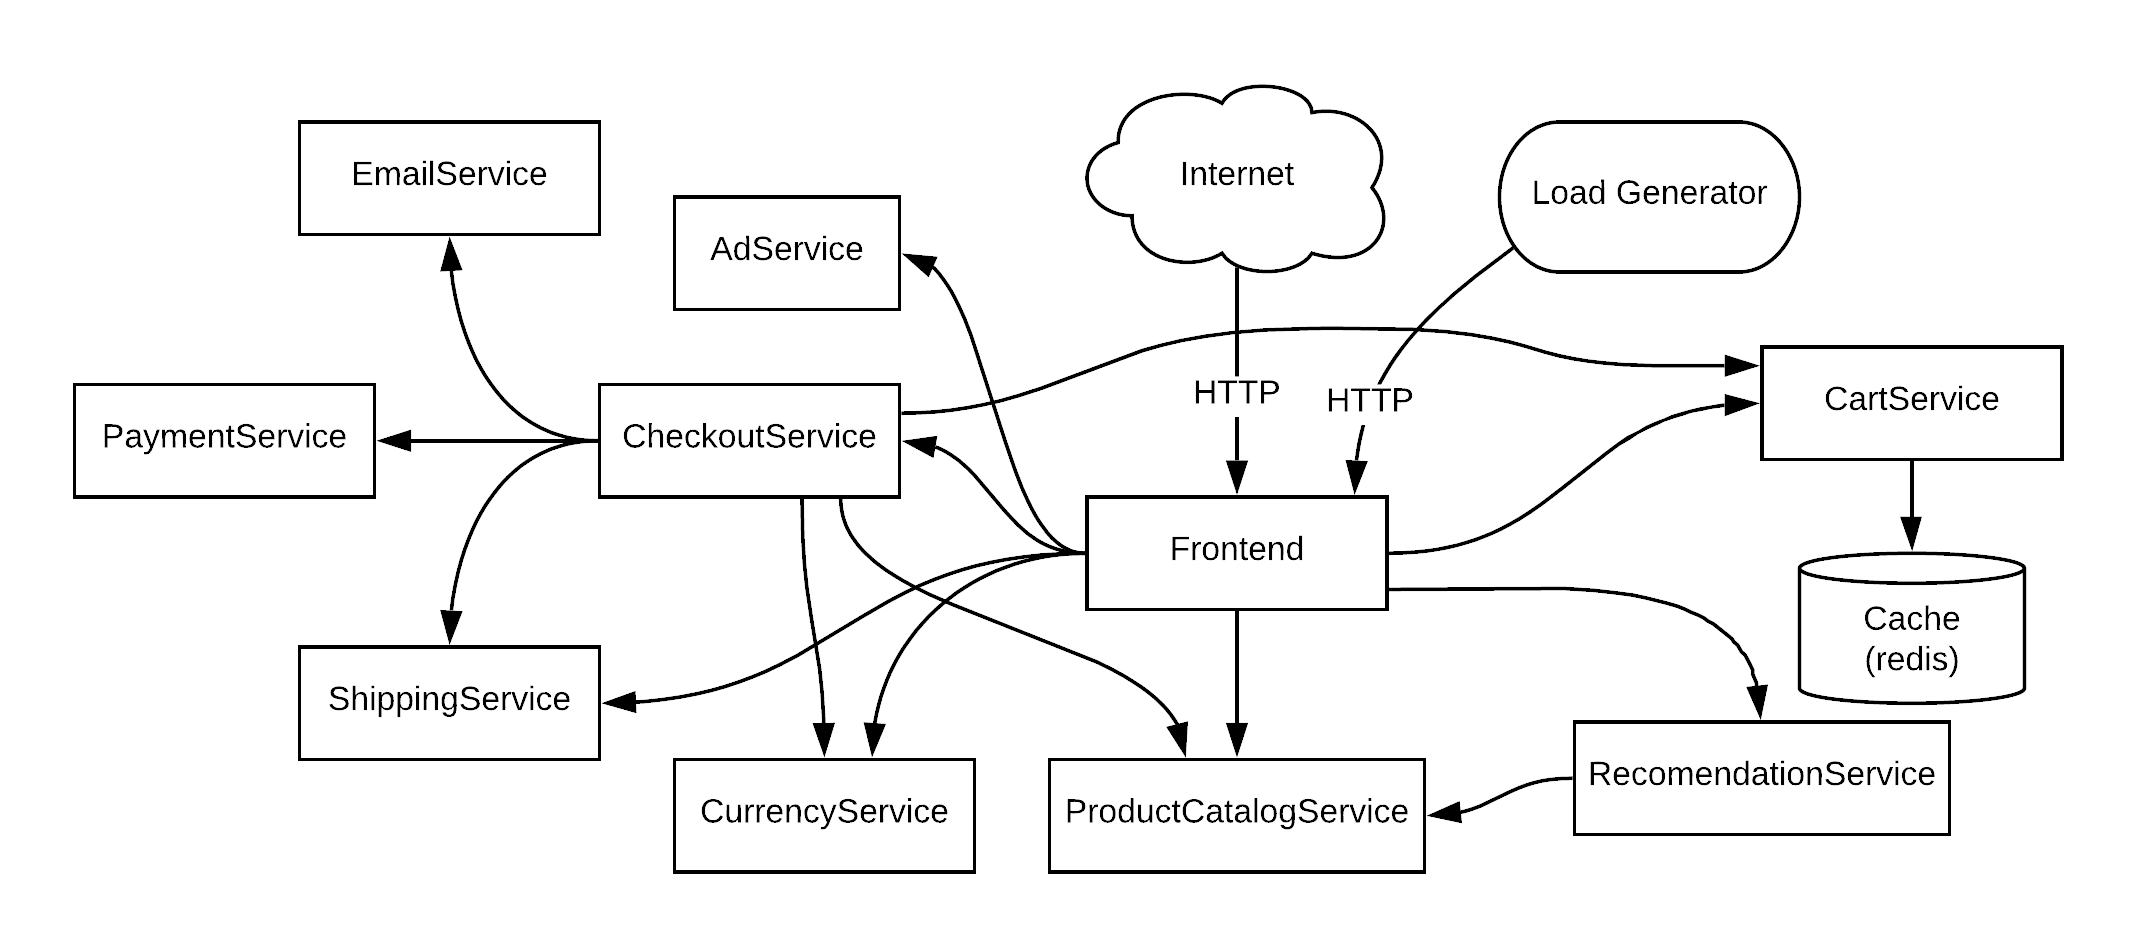
\includegraphics[width=1\textwidth]{resources/ch4/hipster-arch.png}
	\caption{Arsitektur aplikasi Hipster Shop}
	\label{butiq-arch}
\end{figure}

\subsection{Metode Pengujian}
Untuk melakukan pengujian pada sistem PRA yang telah dibuat, \textit{service} yang ada pada Hipster Shop akan dimodifikasi untuk meniru perilaku dari \textit{service} yang mengalami regresi kinerjan. Ada dua metode utama yang dapat dilakukan untuk membuat perilaku regresi pada \textit{service} yaitu dengan menambahkan perintah \textit{sleep} dan juga menambahkan kalkulasi matematika terutama perhitungan fungsi trigonometri yang membutuhkan banyak usaha dari CPU untuk menyelesaikannya sehingga diharapkan fungsi-fungsi pada sebuah \textit{service} akan memiliki \textit{latency} yang lebih besar. 


\subsection{Hasil Pengujian}
Berikut adalah hasil pengujian yang telah dilakukan pada sistem PRA.
